% Main chapter title
\chapter{Hauptkomponentenanalyse}

% Chapter label
\label{pca}

To Do: Kovarianzmatrix / Stichprobenkovarianzmatrix einheitlich!
Begriffe wie samples, PCA, oder features erklären, EIGENVALUE = VARIANCE

Die Hauptkomponentenanalyse (Englisch: Principal Component Analysis (PCA)) ist ein weitverbreitetes multivariates statistisches Verfahren zur Dimensionsreduktion. Allgemein zielen derart Verfahren darauf ab, die in einem Datensatz enthaltene Zahl an Variablen zu verringern, ohne dabei die darin enthaltene Information zu verlieren. (Dies mag zunächst widersprüchlich erscheinen, jedoch enthalten Datensätze aufgrund von Korrelationen oft redundante Informationen.) Durch Verringerung der Dimension können umfangreiche Datensätze strukturiert, veranschaulicht und vereinfacht werden. Damit ist das Verfahren Teil der explorativen Statistik, welche Datensätze hinsichtlich ihrer Zusammenhänge analysiert. Die sich ergebende Struktur kann für weitere Analysezwecke ausgenutzt werden.

Aus diesem Grund hat die Hauptkomponentenanalyse in vielen Bereichen erfolgreich Anwendung gefunden. So kann es in der Bildverarbeitung beispielsweise zur Rauschunterdrückung \cite{babu} oder zur Gesichtserkennung \cite{jiang} genutzt werden. Um Bilder für solch ein Verfahren nutzbar zu machen, werden einzelne Pixel oder patches, also lokale Gruppierungen von Pixeln, eines Bildes als Variable interpretiert. Ein weitere Anwendung in diesem Bereich ist die Erkennung handgeschriebener Zahlen, welche zur automatischen Sortierung von Briefen nach Postleitzahl genutzt werden kann \cite{hastie_elements}. An diesem Beispiel lässt es sich besonders gut verdeutlichen, was es heißt, Zusammenhänge zu analysieren und Strukturen auf Daten zu finden. Bei Anwendung einer Dimensionsreduktion auf Bilder handgeschriebener Zahlen hofft man, dass sich zehn verschiedene Gruppierungen (Englisch: Cluster) ergeben, die für die Ziffern 0 bis 9 stehen. Idealerweise gehören alle Datenpunkte im selben Cluster zur selben Ziffer. Außerdem korrespondieren nahe beieinanderliegende Cluster mit Ziffern, die ähnlich aussehen. (Bild?)

Das mathematische Problem der Hauptkomponentenanalyse kann auf verschiedene Weisen beschrieben werden. Zunächst wollen wir es so konstruieren, dass die Idee des minimalen Informationsverlust im Vordergrund steht. Anschließend werden wir das Problem auf eine Singulärwertzerlegung zurückführen, die auch zur effizienten Implementierung genutzt wird. Des Weiteren werden wir die Verbindung zwischen der Hauptkomponenten- und der Regressionsanalyse betrachten und die geometrische Interpretation weiter verdeutlichen. Zu Schluss runden wir das Kapitel mit einigen Erweiterungen sowie theoretischen Aussagen ab.

\section{Konstruktion}

Gegeben sei ein Datensatz mit $n$ Beobachtungen und $p$ Variablen. Die zentrale Idee der Hauptkomponentenanalyse besteht darin, die $p$ bestehenden Variablen in $k$ neue, unkorrelierte Variablen zu überführen. Um eine Reduktion der Dimension, also $k < p$ zu erreichen, müssen die bestehenden Variablen \textit{zusammengefasst} werden. Idealerweise sollte bei diesem Prozess möglichst wenig Information verloren gehen. Als Maß für den Informationsgehalt der Daten wird hierbei die Varianz verwendet. Das heißt, je größer die Varianz einer Variable, desto mehr Information birgt sie und desto \textit{wichtiger} ist sie. Bei der Erkennung von Unterschieden und Strukturen sind Variablen mit niedriger Varianz nicht von Nutzen. 

Um die Dimension zu reduzieren könnte man einfach nach Eigenschaften größter Varianz suchen und alle Variablen unterhalb eines festgelegten Grenzwertes verwerfen. Dieses Vorgehen fällt allgemein unter die Kategorie \textit{feature selection}. Sowohl die Hauptkomponentenanalyse als auch viele weitere Dimensionsreduktionsverfahren verwenden allerdings ein anderes Prinzip. Anstatt Eigenschaften mit hoher Varianz auszuwählen, konstruiert man neue Variablen, die sich aus den Bestehenden zusammensetzen. Variablen mit hoher Varianz werden in der Konstruktion einen größeren Beitrag spielen als solche mit niedriger Varianz. Dieser Ansatz ist der Kategorie \textit{feature extraction} zuzuordnen.

Um dieses Prinzip zu veranschaulichen, wenden wir uns einem simplem Beispiel zu. Gegeben seien simulierte Daten, welche Gewicht und Größe zu 1000 Personen beinhalten. Bei Betrachtung der Abbildung \ref{pca_example_original} fällt schnell auf, dass die beiden Variablen positiv korreliert sind, d.h. prinzipiell erkennt man folgende Tendenz: Je größer eine Person, desto schwerer ist sie. Somit können wir einen Großteil an Information in einer neuen Variable zusammenfassen, die sich aus einer Linearkombination von Gewicht und Größe ergibt. Die Koeffizienten der Linearkombination ergeben sich aus der ersten Hauptachse, welche in Richtung größter Varianz zeigt. Projizieren wir unsere Daten auf die erste Hauptachse erhalten wir eine eindimensionale Darstellung. Somit sind Personen, die ähnliches Gewicht oder Größe haben auch im transformierten Raum nahe beieinander. Nach Transformation können wir in diesem Beispiel noch immer knapp 90\% der Varianz des ursprünglichen Datensatzes erklären.\\

\begin{figure}
\centering
	\begin{subfigure}{0.45\textwidth}
	\centering
	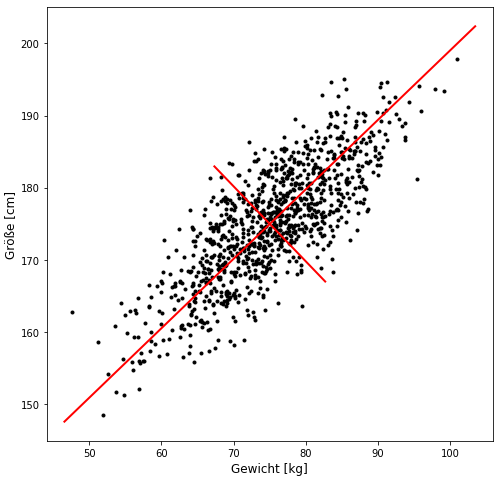
\includegraphics[width = .95\textwidth]{figures/pca_example.png}
	\caption{Simulierte Daten zu Gewicht [kg] und Größe [cm] für 1000 Personen}
	\label{pca_example_original}
	\end{subfigure}
	%	
	\begin{subfigure}{0.45\textwidth}
	\centering
	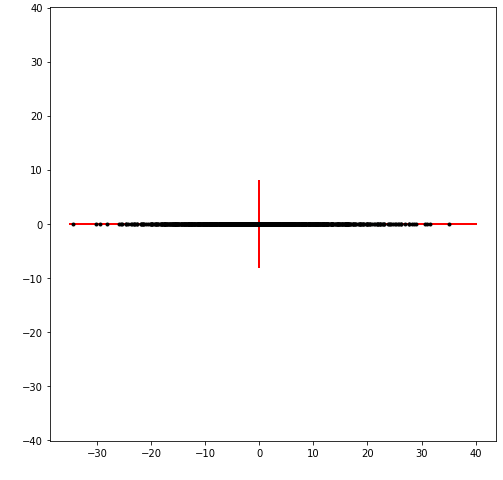
\includegraphics[width = .95\textwidth]{figures/pca_example_rotated.png}
	\caption{Daten nach der Transformation auf die erste Hauptachse}
	\label{pca_example_rotated}
	\end{subfigure}
\caption{Die Abbildung zeigt das Ergebnis einer Hauptkomponentenanalyse auf simulierten Daten. Die roten Linien stellen die beiden Hauptachsen, also die Richtungen größter Varianz des Datensatzes dar. Diese sind nach Konstruktion orthogonal.}
\label{pca_example}
\end{figure}

\textbf{Vorverarbeitung der Daten}

Bevor wir die Hauptkomponentenanalyse auf einen Datensatz anwenden, gibt es einen wichtigen Bearbeitungsschritt zu beachten. Wenn eine Variable weniger variiert als eine Andere aufgrund der verwendeten Einheit oder Skala kann dies zu ungewollten Ergebnissen führen. (REF?) Ohne eine Vorbehandlung der Daten hat so im obigen Beispiel eine Änderung von 1cm die gleiche Bedeutung wie eine Änderung von 1kg.  Daher werden die Daten häufig einem Vorverarbeitungsschritt (Englisch: \textit{preprocessing}) unterzogen. Ein zu diesem Zweck oft verwendetes Verfahren ist die Standardisierung oder auch z-Transformation genannt. Hierbei werden die Variablen $X_i$ zentriert und anschließend auf Einheits-Varianz gebracht. Dies wird erreicht, indem man $X_i$ durch $\frac{X_i - \operatorname{E}[X_i]}{\sqrt{\operatorname{Var}[X_i]}}$ ersetzt. Mathematisch gesehen wendet man das Verfahren somit anstatt der Kovarianzmatrix auf die Korrelationsmatrix an.

\subsection{Problemformulierung als Varianzmaximierung}

Wir wollen nun die Intuition des minimalen Informationsverlust mathematisch beschreiben. Gegeben sei dazu eine Matrix $\mat{X} \in \mathbb{R}^{n\times p}$, wobei $n$ die Anzahl der Beobachtungen und $p$ die Anzahl der Variablen ist. Für eine simplere Darstellung nehmen wir im Folgenden an, dass die Variablen zuvor zentriert wurden. Aufgabe der Hauptkomponentenanalyse ist es nun sukzessive Richtungen größter Varianz zu finden, die sog. \textit{Hauptachsen}. Die Koeffizienten spiegeln dabei den Beitrag jeder einzelnen Variable zur Hauptachse wider. Anschließend werden die \textit{Hauptkomponenten} definiert, welche die Darstellung der Daten bezüglich der neuen Hauptachsen sind. Wir erhalten die erste Hauptachse, indem wir die Varianz von $Z_1 = \mat{X}v_1$, der ersten Hauptkomponente, maximieren, d.h.
\begin{align}
\label{pca_variance_maximization_first}
v_1 = \argmax_{\norm{v}_2 = 1} v^T \mat{\Sigma} v
\end{align}
wobei $\mat{\Sigma} = \frac{\mat{X}^T\mat{X}}{n-1}$ die Stichprobenkovarianzmatrix ist. Die restlichen Hauptachsen können nun sukzessive definiert werden
\begin{align}
\label{pca_variance_maximization_rest}
\begin{split}
v_{i+1} = \argmax_{\norm{v} = 1} v^T \mat{\Sigma} v\\
v_{i+1}^Tv_l = 0 \quad \forall 1 \leq l \leq i
\end{split}
\end{align}
Man sucht also unter den Richtungen, die orthogonal zu allen bisherigen Hauptachsen sind, diejenige, die die Varianz maximiert. Durch Projektion der Daten $Z_i = \mat{X}v_i$ erhält man dann die Hauptkomponenten \cite{vidal}.

Aufgrund der schrittweisen Konstruktion gibt es eine natürliche Ordnung der Hauptkomponenten. Da keine Restriktion an die erste Hauptachse gestellt wird, erklärt die erste Hauptkomponente den größten Teil der Varianz des Datensatzes. Weitere Hauptachsen müssen orthogonal zu den Vorherigen sein und können somit nur einen geringeren Anteil erklären. Ab einem gewissen Punkt erhalten wir durch Berechnung einer weiteren Hauptkomponente also nur geringfügig mehr Information über den Datensatz. Es gilt einen Punkt der Balance zwischen erklärter Varianz und Modellkomplexität zu finden. Mit dieser Fragestellung werden wir uns weiter in Abschnitt \ref{selection_principal_components} beschäftigen.

Für die Maximierungsprobleme (\ref{pca_variance_maximization_first}) und (\ref{pca_variance_maximization_rest}) existiert eine erstaunlich einfache Lösung. Leiten wir (\ref{pca_variance_maximization_first}) in der Langrange-Form $v^T\mat{\Sigma}v + \lambda (1-v^Tv)$ nach $v$ ab und setzen diese gleich Null, erhalten wir den stationären Punkt $\mat{\Sigma}v_1 = \lambda_1 v_1$. Das bedeutet, dass die erste Hauptachse genau dem Eigenvektor des größten Eigenwertes $\lambda_1$ der Stichprobenkovarianzmatrix $\mat \Sigma$ entspricht. Durch Linksmultiplikation mit $v_1^T$ sehen wir, dass durch 
$v_1^T\mat{\Sigma}v_1 = \lambda_1$ die Varianz der ersten Hauptkomponente  gegeben ist. Analog zeigt man, dass auch die folgenden Hauptachsen, die durch (\ref{pca_variance_maximization_rest}) definiert sind, den Eigenvektoren von $\mat \Sigma$ entsprechen \cite{bishop}.

Daher können wir anstatt sukzessiver Berechnung einzelner Hauptachsen die Matrix $\mat{\Sigma}$ direkt diagonalisieren. Aufgrund der Symmetrie von $\mat \Sigma$ können wir eine Eigenwertzerlegung wie in Abschnitt \ref{matrix_decomposition} angeben:
$$\mat{\Sigma} = \frac{1}{n-1}\mat V \mat L \mat{V}^T$$
wobei $\mat{L}$ eine Diagonalmatrix mit Eigenwerten $\lambda_i$ und $\mat V$ die Matrix der Eigenvektoren ist. Somit können die Hauptachsen direkt aus $\mat V$ abgelesen werden. Die Projektion der Daten auf die Hauptachsen wird dann wie zuvor durch Multiplikation der Beobachtungen mit den Eigenvektoren erreicht. 
$$\mat Z = \mat X \mat V$$
Die $i$-te Spalte in $\mat{Z}$ entspricht also der $i$-ten Hauptkomponente und die einzelnen Beobachtungen bezüglich der neuen Darstellung sind die Zeilen von $\mat{Z}$.

Es gibt einen engen Zusammenhang zwischen der Eigenwertzerlegung von $\mat X^T \mat X$ und der Singulärwertzerlegung von $\mat X$. Diese Beziehung können wir nutzen, um die Lösung noch einfacher zu gestalten. Eine Singulärwertzerlegung ergibt
$$\mat{X} = \mat{U}\mat{D}\mat{V}^T$$
wobei $\mat{D}$ die Diagonalmatrix der Singulärwerte, $\mat{U}$ eine orthogonale $n \times n$ und $\mat{V}$ eine orthogonale $p \times p$ Matrix ist. Nun sieht man aufgrund der Orthogonalität von $\mat U$, dass
$$\mat{\Sigma} = \frac{1}{n-1}\mat X^T \mat X = \frac{1}{n-1}\mat{V}\mat{D}\mat{U}^T \mat{U}\mat{D}\mat{V}^T = \frac{1}{n-1}\mat V \mat{D}^2 \mat V^T.$$
Die Singulärwerte stehen also durch $d_i^2 = \lambda_i$ in Beziehung mit den Eigenvektoren von $\mat \Sigma$. 

Zusammengefasst können also alle relevanten Ergebnisse einer Hauptkomponentenanalyse mithilfe einer einzelnen Singulärwertzerlegung von $\mat X$ angegeben werden. Die Hauptachsen entsprechen den Eigenvektoren in $\mat V$, die Hauptkomponenten der Matrix $\mat Z = \mat X \mat V = \mat U \mat D$ und die zugehörigen Varianzen sind durch $d_i^2$ gegeben. Für die Berechnung einer solchen Zerlegung stehen äußert effiziente Verfahren zur Verfügung, welche sowohl den $n<p$ als auch den $p<n$ Fall schnell in $\mathcal{O}(np \cdot \min\{n,p\})$ lösen können. 

(So können wir eine Hauptkomponentenanalyse  durchführen. In der Praxis wird meist nur die kompakte Singulärwertzerlegung, die nur von Null verschiedene Singulärwerte berücksichtigt, berechnet. Die Anzahl ist gegeben durch den Rang von $\mat X$Es sei $k \leq \min\{n,p\}$ der Rang von $\mat X$.)

\subsection{Formulierung als Regressionsproblem}

Wir widmen uns nun einer anderen Sichtweise auf die Hauptkomponentenanalyse, welche einen Zusammenhang zur linearen Regression herstellt und eine geometrische Interpretation ermöglicht. Hierbei möchte man einen $k$-dimensionalen Unterraum finden, der die Daten bestmöglich approximiert wenn sie darauf projiziert werden. Mathematisch ausgedrückt minimieren wir also die Residuen der Projektion.

Sei dazu $x_i$ die $i$-te Beobachtung, also die $i$-te Zeile von $\mat X$ und $\mat V_k = \begin{bmatrix} v_1 & \cdots & v_k \end{bmatrix}$ eine $p \times k$ orthonormale Matrix. Wie in Abschnitt \ref{orthogonality} beschrieben wird durch den Operator $\mat V_k \mat V_k^T$ jede Beobachtung orthogonal auf den durch $V_1, \ldots , V_k$ aufgespannten Unterraum projiziert. Eine bestmögliche $\ell_2$-Approximation der Daten ist gegeben wenn wir die Distanz zwischen jeder Beobachtung und seiner Projektion minimieren \cite{zou_sparsepca}:
\begin{align}
\label{pca_regression_formulation}
\begin{split}
\mat{\widehat{V}}_k = \argmin_{\mat{V}_k} \sum_{i=1}^{n} \norm{x_i - \mat{V}_k \mat{V}_k^Tx_i}_2^2\\
\mat{V}_k^T\mat{V}_k = I_{k \times k}
\end{split}
\end{align}
Ein mathematisch rigoroser Beweis, dass die Lösung von (\ref{pca_regression_formulation}) genau den ersten $k$ Hauptachsen entspricht, befindet sich in \cite{vidal}. Wir möchten hier eine intuitive Erklärung für diese Äquivalenz geben. Wenn wir von der Varianz eines Datensatzes sprechen, reden wir von der Summe der Varianzen der einzelnen Variablen. Somit ist die Gesamtvarianz durch $\frac{1}{n-1}\norm{\mat X}_{F}^{2}$ gegeben. Mithilfe des verallgemeinerten Satzes von Pythagoras erhalten wir
\begin{align*}
\norm{\mat X}_{F}^{2} & = \sum_{i=1}^{n} \norm{x_i}_{2}^{2}\\
& = \sum_{i=1}^{n} \norm{x_i - \mat V_k \mat V_k^T x_i + \mat V_k \mat V_k^T x_i}_{2}^{2}\\
& = \sum_{i=1}^{n} \norm{x_i - \mat V_k \mat V_k^T x_i}_2^2 + \norm{\mat V_k \mat V_k^T x_i}_{2}^{2}\\
& = \norm{\mat X - \mat X \mat V_k \mat V_k^T}_{F}^{2} + \norm{\mat X \mat V_k \mat V_k^T}_{F}^{2}.
\end{align*}
Weiter sehen wir, dass
\begin{align*}
\norm{\mat X \mat V_k \mat V_k^T}_{F}^{2} & = \spur{\mat X \mat V_k \mat V_k^T (\mat X \mat V_k \mat V_k^T)^T}\\
& = \spur{\mat V_k^T \mat X^T \mat X \mat V_k}\\
& = \sum_{i=1}^{k} v_i^T (\mat X^T \mat X) v_i
\end{align*}
In (\ref{pca_variance_maximization_first}) und (\ref{pca_variance_maximization_rest}) haben wir den Term $v_i^T \mat \Sigma v_i$, der die Varianz der $i$-ten Hauptkomponente beschreibt, sequentiell maximiert. Drücken wir (\ref{pca_variance_maximization_first}) und (\ref{pca_variance_maximization_rest}) in einem gemeinsamen Berechnungsproblem aus ergibt sich
\begin{align}
\label{pca_variance_maximization}
\begin{split}
\widehat{\mat V}_k = \argmax_{\mat V_k}\sum_{i=1}^{k} v_i^T \mat \Sigma v_i\\
\mat V_k^T\mat V_k = \mat I_{k \times k}
\end{split}
\end{align}
Kommen wir nun zurück auf die Zerlegung der Gesamtvarianz
\begin{align*}
\frac{1}{n-1}\norm{\mat X}_{F}^{2} = \frac{1}{n-1}\norm{\mat X - \mat X \mat V_k \mat V_k^T}_{F}^{2} + \sum_{i=1}^{k} v_i^T \mat \Sigma v_i
\end{align*} 
Mathematisch gesehen macht es keinen Unterschied, ob wir die Varianz der Hauptkomponenten $\sum_{i=1}^{k} v_i^T \mat \Sigma v_i$ maximieren oder die Residuen der Projektion $\frac{1}{n-1}\norm{\mat X - \mat X \mat V_k \mat V_k^T}_{F}^{2}$ minimieren. Diese Idee ist geometrisch in Abbildung \ref{pca_projection_explanation} veranschaulicht. Hierbei versucht man im ersten Fall eine Hauptachse durch den Datensatz zu finden, so dass die Varianz entlang dieser maximiert werden. Anders versucht man im zweitem Fall eine Hauptachse zu finden, so dass die Summe der Distanzen zwischen Datenpunkt und seiner Projektion minimiert wird.
\begin{figure}
\centering
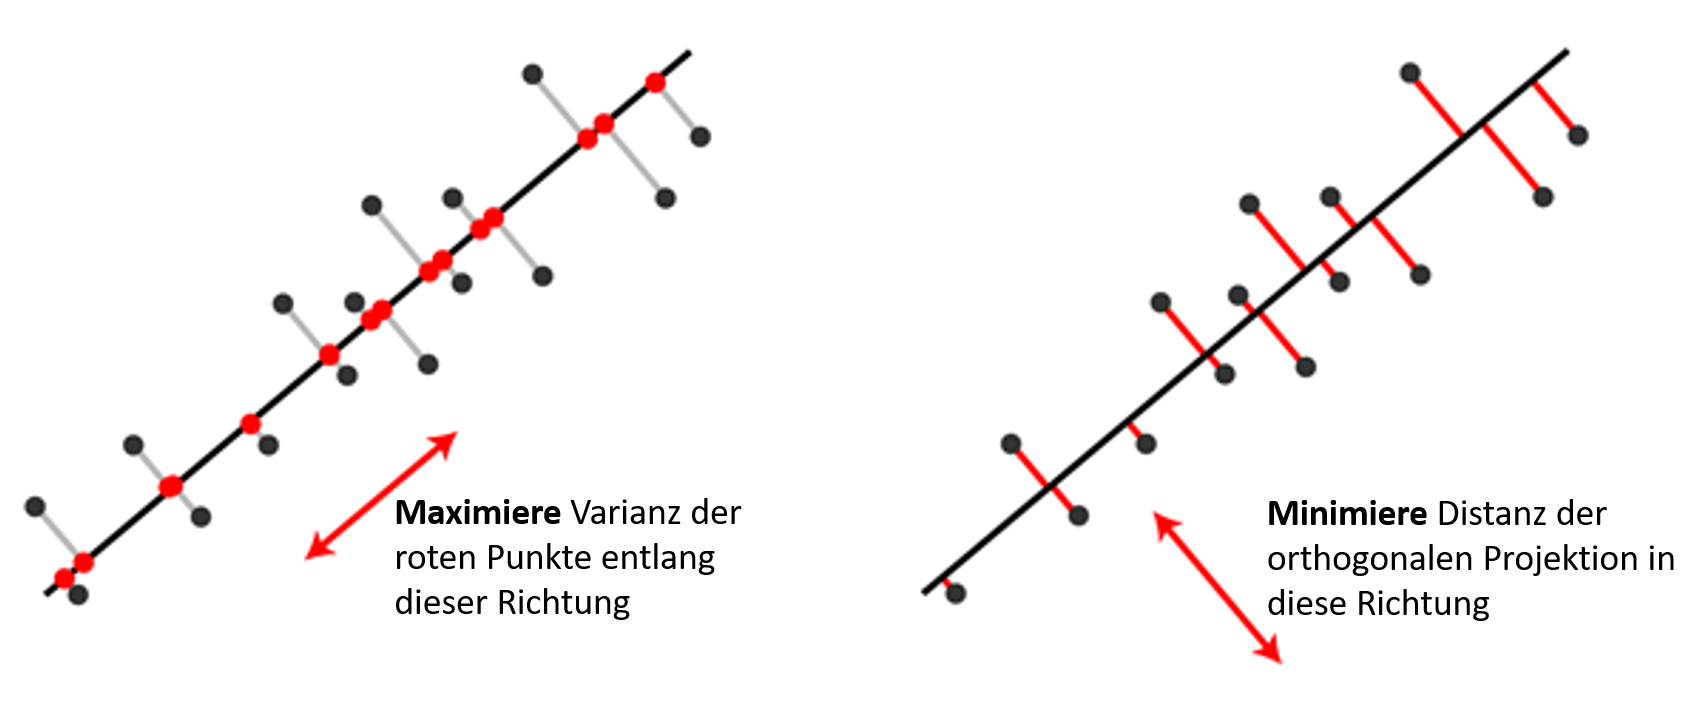
\includegraphics[width = 0.8\textwidth]{figures/pca_projection_explanation_german.png}
\caption{Die Abbildung zeigt die Äquivalenz von Maximierung der Varianz und Minimierung der Residuen in zwei Dimensionen.}
\label{pca_projection_explanation}
\end{figure} 

Da die Daten auf den niedrigdimensionaleren Raum linear transformiert werden gehört die Hauptkomponentenanalyse zu den linearen Dimensionsreduktionsverfahren. Anhand von (\ref{pca_regression_formulation}) erkennt man zudem einen starken Zusammenhang zur linearen Regression, bei welcher ebenfalls die Summe der Residuenquadrate minimiert werden. Neben der unterschiedlichen Motivation der beiden Verfahren liegt die entscheidende Differenz in der Art der Projektion. Während bei linearer Regression die Projektion orthogonal bezüglich der unabhängigen Koordinatenachsen ist, werden die Daten bei der Hauptkomponentenanalyse orthogonal auf die Hauptachsen projiziert. Ausgehend von (\ref{pca_regression_formulation}) werden wir im nächsten Kapitel die Variante der dünnbesetzten Hauptkomponentenanalyse beschreiben.

\subsection{Weitere Formulierungen} 

Wir werden nun kurz auf zwei weiteren Formulierungen eingehen anhand welcher weitere Eigenschaften der Hauptkomponentenanalyse deutlich werden. Da $\mat Z_k = \mat X \mat V_k$ die ersten $k$ Hauptkomponenten beinhaltet, kann (\ref{pca_regression_formulation}) auch geschrieben werden als
\begin{align}
\label{pca_minimize_reconstruction_error}
\begin{split}
(\widehat{\mat{Z}}_k, \widehat{\mat V}_k) = \argmin_{\mat Z_k, \mat V_k} \norm{\mat X - \mat Z_k \mat V_k^T}_{F}^{2}\\
\mat V_k^T\mat V_k = \mat I_{k \times k}.
\end{split}
\end{align}
Durch $\mat Z_k \mat V_k^T$ ist also eine bestmögliche Rekonstruktion der Datenmatrix $X$ gegeben. In anderen Worten wird in (\ref{pca_minimize_reconstruction_error}) also der $\ell_2$-Rekonstruktionsfehler minimiert. Diese Formulierung werden wir als Grundlage für Verallgemeinerungen der Hauptkomponentenanalyse in Abschnitt \ref{pca_extensions} wählen.

Wir haben bereits gesehen, dass die abgeschnittene Singulärwertzerlegung $\mat X_k = \mat U_k \mat D_k \mat{V}_k^T \in \mathbb{R}^{n \times k}$ die optimale Lösung für die Hauptkomponentenanalyse liefert. Diese ist aufgrund des Eckart-Young-Mirsky-Theorem, welches wir bereits in Abschnitt \ref{matrix_approximation} kennengelernt haben, Lösung des Problems
\begin{align}
\begin{split}
\widehat{\mat X}_k = \argmin_{\mat X_k} \norm{\mat X - \mat X_k}_F^2\\
\rang{\mat X_k} \leq k.
\end{split}
\end{align}
Somit ist $\widehat{\mat X}_k$ diejenige Matrix mit Rang $k$, die $X$ am Besten approximiert. Die Rang-Bedingung legt also die Komplexität des Modells fest.

\section{Selektion der Hauptkomponenten}
\label{selection_principal_components}

Die Frage nach der Wahl der Komplexität eines Modells ist nicht immer einfach zu beantworten. Auch bei Dimensionsreduktionsverfahren kennen wir oft die intrinsische Dimension unserer Daten a priori nicht. Daher ist es schwer zu sagen, wie viele Hauptkomponenten benötigt werden, um die Daten geeignet zu modellieren. Es gilt einen Punkt der Balance zwischen kleinem Rekonstruktionsfehler und starker Dimensionsreduktion $k \ll \min\{n, p\}$ zu finden. 

Aufgrund der einfachen Lösung der Hauptkomponentenanalyse wählt man oft den Ansatz zunächst alle $k = \min\{n, p\}$ Hauptkomponenten zu berechnen. Selbst für große $n$ und $p$ stehen effiziente Algorithmen zur Verfügung. Anschließend bewertet man die Ergebnisse anhand der erklärten Varianz $\lambda_i$ jeder Hauptkomponente. 

Meist wird eine Faustregel herangezogen. Eine simple Methode wäre so viele Hauptkomponenten auszuwählen, damit insgesamt ein vorher festgelegter Wert (z.B. 90\%) der Varianz erhalten bleibt. Bildliche Darstellung der Varianzen (vgl. Abbildung) werden in einem sog. \textit{scree plot} dargestellt. In manchen Fällen gibt es eine klare Trennung in der Größe der Eigenwerte. CITE schlagen vor nach einem starkem Knick in der Kurve zu suchen. Allerdings sind dieser Art Verfahren sehr subjektiv, da es einen solchen Knick nicht zwangsläufig geben muss bzw. es auch mehrere geben kann.

Die eigentliche Dimensionsreduktion findet dann durch Selektion statt. Je nach Komplexität des Modells, welches man erreichen möchte, können so mehr oder weniger Hauptkomponenten ausgewählt werden. Je mehr Hauptkomponenten man auswählt, desto mehr Information erhält man über den Datensatz. Allerdings wird das Modell mit steigender Anzahl an Variablen immer komplizierter. Es gilt einen Punkt der Balance zu finden, der ein gutes Mittel aus Information und Komplexität liefert. Dieser kann vom Anwendungsfall abhängen. 

Abbildung Scree Plot

Optimal singular threshold \cite{gavish}

\section{Grenzen der Anwendbarkeit} \label{theo_results}

Obwohl die Hauptkomponentenanalyse in vielen Situationen helfen kann, Datensätze zu veranschaulichen und zu strukturieren, gibt es keine Garantie für sinnvolle Ergebnisse. Im Folgendem werden wir Szenarien beschreiben, bei denen unerwünschte Effekte bei der Verwendung dieses Verfahrens auftreten. Daher gilt es den Datensatz vorerst hinsichtlich folgender Gesichtspunkte zu untersuchen: 

\begin{itemize}
\item Lineare Beziehung zwischen Variablen
\item Korrelation der Variablen
\item Vollständigkeit des Datensatzes
\item Ausreißer in den Daten
\item Anzahl an Beobachtungen in Relation zu Anzahl an Variablen
\end{itemize}

Wie in REF beschrieben versuchen wir Daten in einen niedrigdimensionaleren linearen oder affinen Unterraum zu transformieren. Es kann aber durchaus vorkommen, dass es keine lineare Beziehung zwischen den Variablen gibt. Nichtlineare Strukturen können von PCA nicht erfasst werden und gehen somit verloren. \cite{vidal} Vidal et al. zeigen diese Grenze konkret am Beispiel von Porträt-Fotos auf. Seit der Entstehung von PCA gab es aber zahlreiche nicht-lineare Erweiterungen. So nutzt zum Beispiel Kernel PCA den \textit{Kernel Trick} aus, bei welchem man die Daten zuerst durch eine nichtlineare Transformation in ein höherdimensionalen Raum einbettet von dem man sich erhofft, dass die Daten in diesem linear verteilt. Erst anschließend wird dann die eigentliche Reduktion durchgeführt. Hierbei muss man die Daten aber nicht im höherdimensionalen Raum auswerten. CITE. Andere Erweiterungen, die allgemein unter \textit{manifold learning} zusammengefasst werden können, basieren auf der Idee, dass die Dimension des Datensatz nur künstlich hoch ist. Man versucht die lokale Geometrie der Mannigfaltigkeit (Begriff erklären?) zu approximieren und damit direkt eine niedrigdimensionale Einbettung zu erhalten. Hierunter fallen zum Beispiel die multidimensionale Skalierung oder ISOMAP.

Damit der Datensatz für eine Dimensionsreduktion per PCA geeignet ist, müssen die verschiedenen Variablen einen gewissen Grad an Korrelation aufweisen. Im extremen Fall der Unabhängigkeit der Variablen bewirkt eine Hauptachsentransformation nichts. Reduziert man dann die Anzahl der Hauptkomponenten verliert man mit jeder Variable einen Großteil der Information.

Ein weiterer Gesichtspunkt ist die Vollständigkeit eines Datensatzes. Finden wir fehlende oder korrupte Einträge in unserem Datensatz vor, kann die klassische Hauptkomponentenanalyse ... . Für dieser Art Probleme existieren entsprechende Ergänzungen von PCA wie zum Beispiel in cite und cite. Ausreißer in den Daten können die Resultate drastisch beeinflussen. Genaue Effekte überlegen und CITE. Aus diesem Grund sollten Ausreißer vor der Anwendung von PCA entfernt werden.

Ausreißer in den Daten.

Anzahl der Variablen zu hoch.

Darüber hinaus gibt es noch eine Reihe Spezialfälle, bei denen Probleme auftreten können. So kann es zum Beispiel passieren, dass die relevanten Informationen in den Variablen mit niedriger Varianz versteckt sind. Da die Hauptkomponentenanalyse gerade diese Variablen vernachlässigt, wird sich unter Umständen nicht die erwünschte Struktur auf den Daten ergeben. Es bedarf anderer Methoden mit anderen Ansätzen, um eine Dimensionsreduktion zu ermöglichen. Oftmals weiß man aber im Vorhinein nicht, in welchen Variablen diese Unterscheidungsmöglichkeit versteckt ist.

Das wohl wichtigste/größte Hindernis im Zuge dieser Arbeit ist sicherlich die durch die Transformation entstehenden Interpretationsschwierigkeiten. Jede Hauptkomponente entsteht wie oben beschrieben durch eine Linearkombination der Ausgangsvariablen. Während die Ausgangsvariablen Bedeutungen wie Gewicht oder Größe hatten ist in vor allem in hochdimensionalen Fällen eine Interpretation der Hauptkomponenten nur schwer möglich (Rotation Techniques CITE). Dieser Interpretationsverlust ist Ausgangspunkt der Idee der dünnbesetzten Hauptkomponentenanalyse, genannt sparse PCA. Diesem Verfahren ist das folgende Kapitel gewidmet.

\section{Erweiterungen der Hauptkomponentenanalyse}
\label{pca_extensions}
Wie wir bereits gesehen haben, gibt es viele verschiedene Erweiterungen von PCA. Die meisten kann man unter folgendem Schema zusammenfassen: (Welche genau?)

$$\min_{\mat{Z},\mat{V}} \underbrace{\norm{\mat{X} - \mat{Z}\mat{V}^T}_F}_{\text{Loss Function}} + \underbrace{\lambda_z f_z(\mat Z) + \lambda_v f_v(\mat V)}_{\text{Regularisierung}}$$
$$\text{subject to} \quad \underbrace{\mat Z \in \Omega_z, \mat V \in \Omega_v}_{\text{Nebenbedingungen}}$$

\begin{table}
\centering
\begin{tabular}[c]{lll}
\thead{Loss Functions} & \thead{regularizer} & \thead{constraints} \\
\hline
\makecell{quadratic\\(real data)} & \makecell{L2 norm\\(small factors)} & \makecell{Nonnegative\\(additive factors)}\\
\makecell{absolute\\(robust to outliers)} & \makecell{L1 norm\\(sparse factors)}\\
\makecell{logistic\\(binary data)} & \makecell{Derivative penalties\\ (smooth factors)}\\
\makecell{Poisson\\(integer data)}\\
\makecell{circular\\(angular data)}\\
\end{tabular}
\caption{Allgemeines Schema zu PCA Erweiterungen}
\end{table}

\section{Theoretische Aussagen}
\label{pca_theorems}

PCA Variablen sind unkorelliert und die Loadings orthogonal. Liegt wahrscheinlich daran, dass wie die Eigenvektoren für symmetrische Matrizen $\mat X^{\top}\mat X$ orthogonal sind und die Kovarianzmatrix der Hauptkomponenten $(\mat X \mat V)^{\top}\mat X \mat V = \mat V^{\top}\mat{\Sigma} \mat V$ eine Diagonalmatrix ist.

non convex problem that can be solved efficiently by truncated SVD.

Baldi Hornik 1989
all local minima are solutions to pca
all non optimal critical points are saddle points or maxima

\begin{thm}
PCA always gives unique solution.
\end{thm}

\begin{thm}[\cite{vidal}]
Sei $\mat X \in \mathbb{R}^n$ und $\mat A_{p,k} = [\alpha_1, \ldots \alpha_k] $   
\end{thm}

\begin{thm}
PCA inconsistent for n << p.
\end{thm}

